% =====================================================================
\chapter{Esquema eléctrico y cableado}\label{cap:electrico}

\section{Plano histórico}
\begin{figure}[H]
\centering
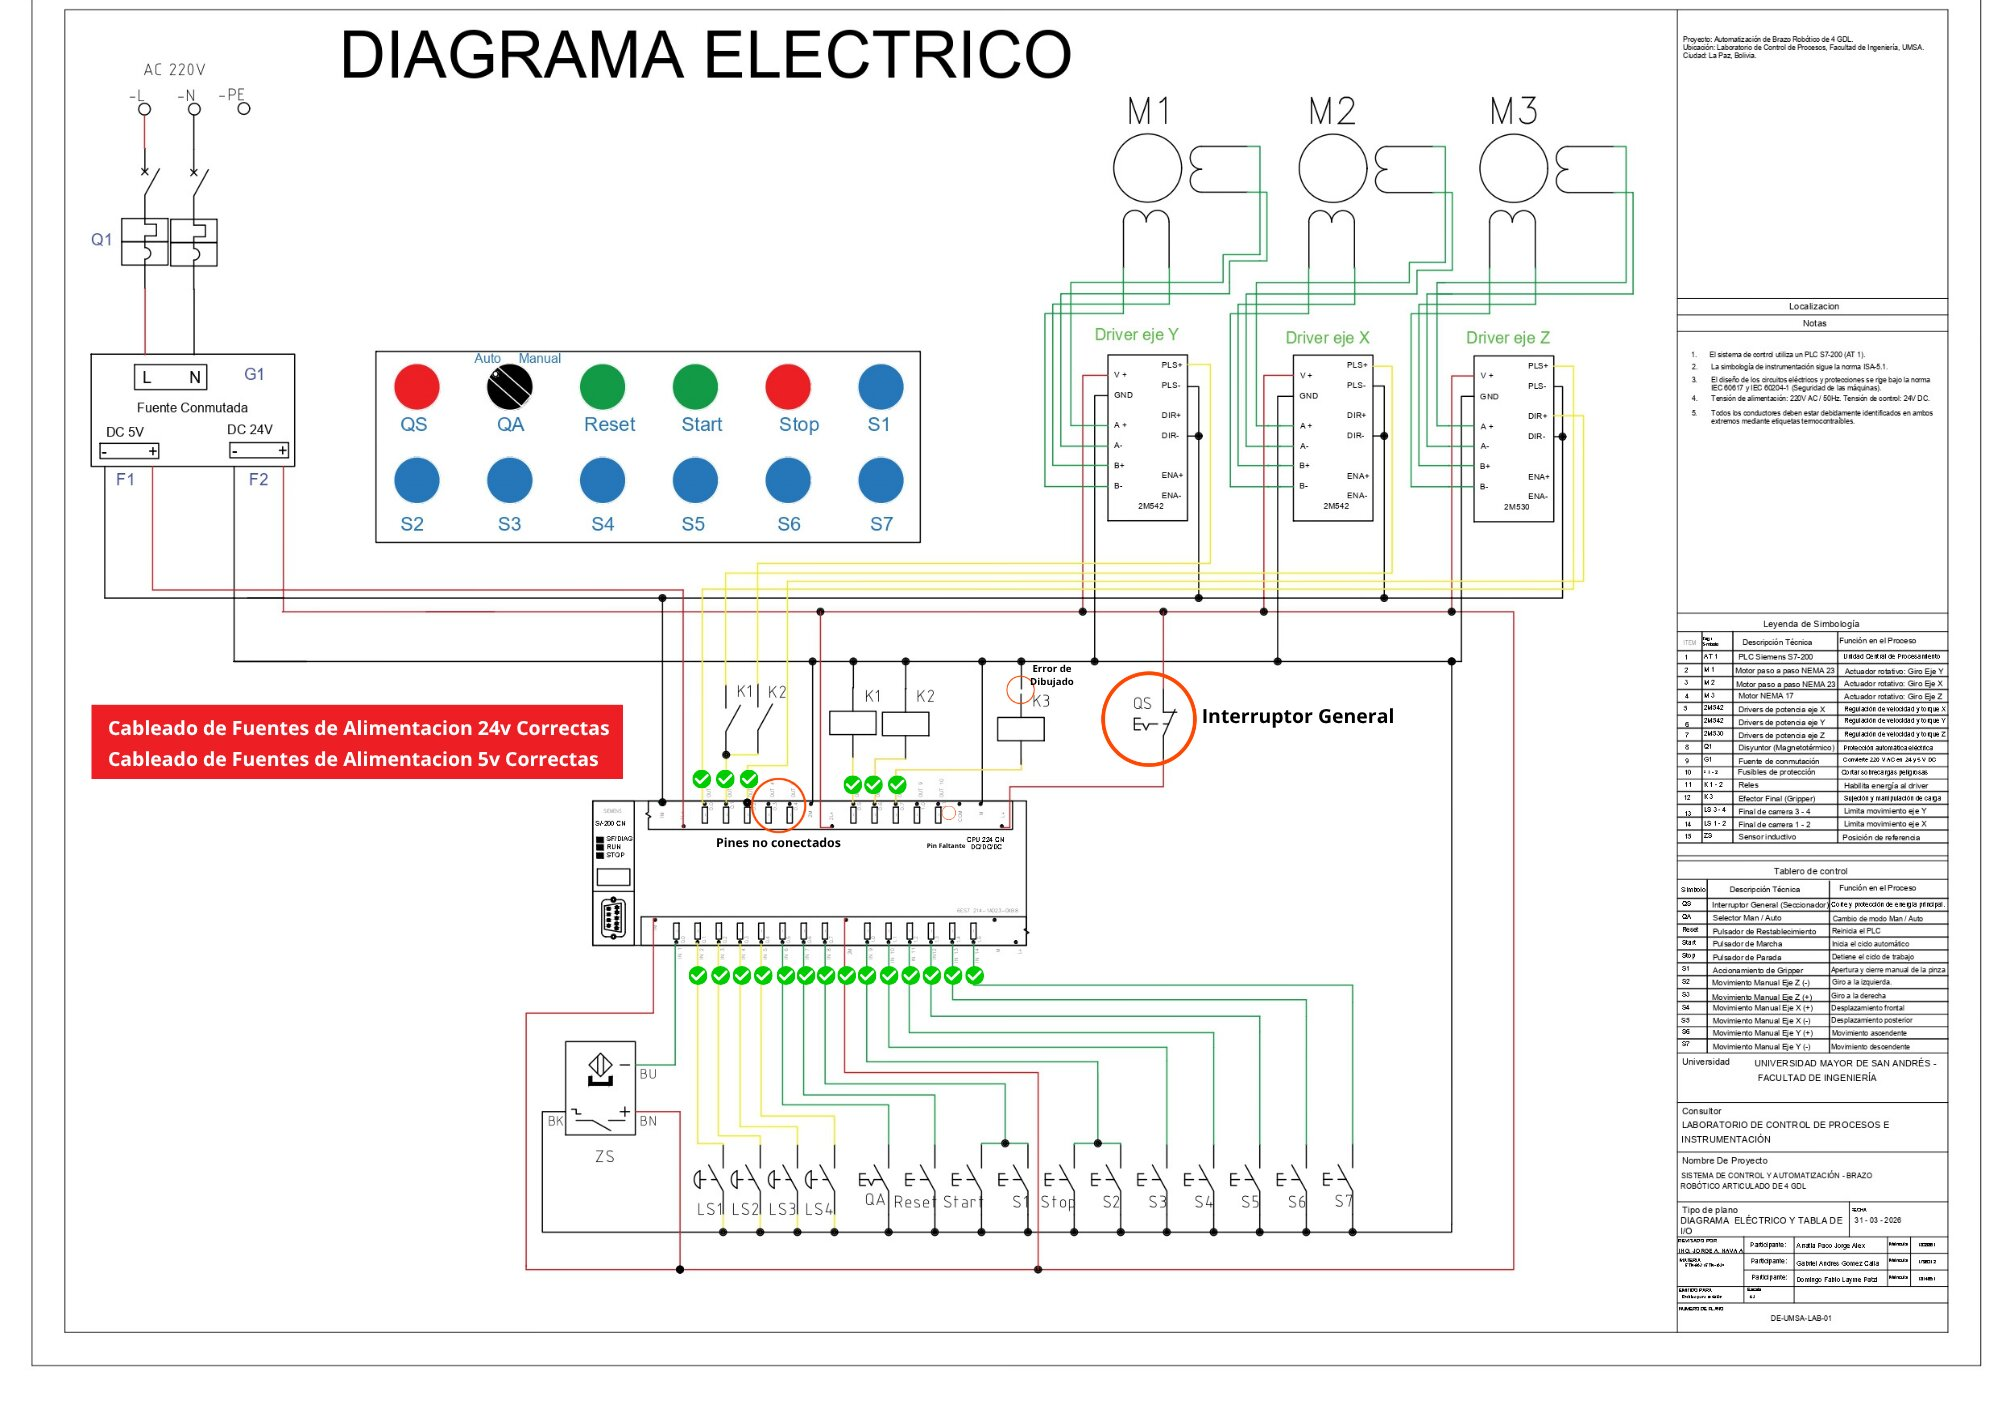
\includegraphics[width=\linewidth]{brazo_electrico_historico_vista.jpg}
\caption{Plano eléctrico heredado (\texttt{planos/electrico/brazo\_electrico\_historico.dwg}). El informe 1 encontró pines sin graficar, DIR+ de X e Y sin conectar y el trazo de la garra equivocado (sección \ref{sec:kaizen}).}
\end{figure}

\section{Etapa de potencia}
\begin{figure}[H]
\centering
\begin{tikzpicture}[node distance=6mm and 9mm]
\node[caja, text width=1.8cm] (red) {red\\220~V AC};
\node[caja, text width=2.6cm, right=of red] (dz) {disyuntor diferencial\\DZ47LE-63\\16~A · 30~mA};
\node[cajan, text width=2.4cm, right=of dz] (f) {fuente conmutada\\24~V / 5~V DC};
\node[caja, text width=2.4cm, right=12mm of f, yshift=14mm] (plc) {PLC CPU 224\\(L+/M 24~V)};
\node[caja, text width=2.4cm, right=12mm of f] (drv) {drivers 2M542 (X, Y)\\y 2M530 (base)\\VDC 24~V};
\node[caja, text width=2.4cm, right=12mm of f, yshift=-14mm] (mando) {sensores, relés\\K1--K3, solenoide};
\draw[flecha] (red) -- (dz); \draw[flecha] (dz) -- (f);
\draw[flecha] (f.east) -- ++(4mm,0) |- (plc.west);
\draw[flecha] (f) -- (drv);
\draw[flecha] (f.east) -- ++(4mm,0) |- (mando.west);
\node[etiq, text width=3.6cm, right=4mm of drv] {los drivers admiten 20--50~V: con 36--48~V el par a alta velocidad mejora (capítulo \ref{cap:drivers})};
\end{tikzpicture}
\caption{Distribución de energía.}
\end{figure}

\section{Etapa de mando}
\begin{figure}[H]
\centering
\begin{tikzpicture}[x=1cm,y=1cm, borne/.style={circle, draw, fill=white, inner sep=1.2pt}, rot/.style={font=\scriptsize\ttfamily, anchor=east}]
% PLC
\draw[thick, fill=naranja!8] (0,0) rectangle (2.4,-10.2);
\node[font=\small\bfseries, align=center] at (1.2,0.45) {PLC S7-200\\CPU 224};
\foreach \y/\t in {-0.6/Q0.0,-1.4/Q0.1,-2.2/Q0.2,-3.0/Q0.3,-3.8/Q0.4,-4.6/Q0.5,-5.4/Q0.6,-6.2/Q0.7}
  {\node[borne] at (2.4,\y) {}; \node[font=\scriptsize\ttfamily, anchor=east] at (2.3,\y) {\t};}
\foreach \y/\t in {-6.9/I0.0,-7.8/I0.1..I0.4,-8.6/I0.5..I0.7,-9.4/I1.0..I1.5}
  {\node[borne] at (0,\y) {}; \node[font=\scriptsize\ttfamily, anchor=west] at (0.1,\y) {\t};}
% relés
\node[draw, fill=gris, minimum width=1.2cm, minimum height=0.8cm, font=\scriptsize] (k1) at (5.2,-4.6) {K1};
\node[draw, fill=gris, minimum width=1.2cm, minimum height=0.8cm, font=\scriptsize] (k2) at (5.2,-5.4) {K2};
\node[draw, fill=gris, minimum width=1.2cm, minimum height=0.8cm, font=\scriptsize] (k3) at (5.2,-6.2) {K3};
\draw[flecha] (2.4,-4.6) -- node[above, etiq]{bobina} (k1); \draw[flecha] (2.4,-5.4) -- (k2); \draw[flecha] (2.4,-6.2) -- (k3);
% drivers
\node[draw, fill=white, minimum width=2.6cm, minimum height=1.5cm, align=center, font=\scriptsize] (dz) at (10.2,-0.9) {\textbf{driver base 2M530}\\PUL \ DIR \ ENA};
\node[draw, fill=white, minimum width=2.6cm, minimum height=1.5cm, align=center, font=\scriptsize] (dx) at (10.2,-2.9) {\textbf{driver X 2M542}\\PUL \ DIR \ ENA};
\node[draw, fill=white, minimum width=2.6cm, minimum height=1.5cm, align=center, font=\scriptsize] (dy) at (10.2,-4.9) {\textbf{driver Y 2M542}\\PUL \ DIR \ ENA};
\draw[thick] (2.4,-0.6) -- (8.9,-0.6) node[pos=0.55, above, etiq]{PUL base};
\draw[thick] (2.4,-2.2) -- (7.6,-2.2) |- (8.9,-1.2) node[pos=0.8, above, etiq]{DIR base};
% Q0.1 por contactos de K1 y K2
\draw[thick] (2.4,-1.4) -- (6.6,-1.4) -- (6.6,-2.6);
\draw[thick] (6.6,-2.6) -- (6.9,-2.6); \draw[thick] (6.9,-2.45) -- (7.2,-2.75); \draw[thick] (7.2,-2.6) -- (8.9,-2.6) node[pos=0.5, above, etiq]{PUL X};
\node[font=\tiny] at (7.05,-2.95) {K1};
\draw[thick] (6.6,-2.6) -- (6.6,-4.6) -- (6.9,-4.6); \draw[thick] (6.9,-4.45) -- (7.2,-4.75); \draw[thick] (7.2,-4.6) -- (8.9,-4.6) node[pos=0.5, above, etiq]{PUL Y};
\node[font=\tiny] at (7.05,-4.95) {K2};
\draw[dashed] (k1.north) -- (7.05,-2.8); \draw[dashed] (k2.north) -- (7.05,-4.8);
\draw[thick] (2.4,-3.0) -- (6.3,-3.0) -- (6.3,-3.2) -- (8.9,-3.2) node[pos=0.6, below, etiq]{DIR X};
\draw[thick] (2.4,-3.8) -- (6.1,-3.8) -- (6.1,-5.2) -- (8.9,-5.2) node[pos=0.8, below, etiq]{DIR Y};
% garra
\node[draw, fill=white, minimum width=2.6cm, minimum height=1cm, align=center, font=\scriptsize] (sol) at (10.2,-6.6) {solenoide de la garra\\24~V DC};
\draw[thick] (k3.east) -- node[above, etiq]{contacto K3, +24~V} (sol.west);
% motores
\node[draw, circle, minimum size=0.9cm, font=\scriptsize, right=6mm of dz] (mz) {M};
\node[draw, circle, minimum size=0.9cm, font=\scriptsize, right=6mm of dx] (mx) {M};
\node[draw, circle, minimum size=0.9cm, font=\scriptsize, right=6mm of dy] (my) {M};
\draw[thick] (dz) -- (mz); \draw[thick] (dx) -- (mx); \draw[thick] (dy) -- (my);
% sensores
\node[draw, fill=white, align=center, font=\scriptsize, text width=3cm, anchor=east] (ind) at (-1.4,-6.75) {inductivo LJ12A3-4-Z/BX\\NPN NA, 3 hilos};
\node[draw, fill=white, align=center, font=\scriptsize, text width=3cm, anchor=east] (fc) at (-1.4,-7.8) {4 finales de carrera};
\node[draw, fill=white, align=center, font=\scriptsize, text width=3cm, anchor=east] (bt) at (-1.4,-9.0) {botonera: selector,\\Stop, Start, S1--S7};
\draw[thick] (ind.east) -- (-0.5,-6.75) -- (-0.5,-6.9) -- (0,-6.9); \draw[thick] (fc) -- (0,-7.8); \draw[thick] (bt.east) -- (-0.7,-9.0) -- (-0.7,-8.6) -- (0,-8.6); \draw[thick] (-0.7,-9.0) -- (-0.7,-9.4) -- (0,-9.4);
\end{tikzpicture}
\caption{Esquema funcional de mando. Q0.1 llega al driver X solo con K1 cerrado y al driver Y solo con K2 cerrado.}
\end{figure}

\nota{\textbf{Este esquema es funcional}: muestra qué señal va a qué componente, verificado con el PLC en marcha. Los bornes exactos, los comunes (1M, 2M, 1L+), el nivel de las entradas PUL/DIR de los drivers (entradas optoacopladas de 5~V, alimentadas desde el riel de 5~V o con resistencias en serie) y la entrada ENA deben tomarse del plano versión 2.0 cuando se termine (guía 2).}

\section{Por qué los relés K1 y K2}
La CPU 224 tiene solo dos generadores de pulsos rápidos, en Q0.0 y Q0.1. Con tres motores, quien diseñó la planta dedicó Q0.0 a la base y repartió Q0.1 entre los dos carros mediante los contactos de K1 y K2. Consecuencias de diseño:
\begin{itemize}
\item X e Y pueden moverse a la vez, pero recibiendo exactamente los mismos pulsos, a la misma frecuencia.
\item Un movimiento con recorridos distintos se divide en un tramo común (K1 y K2 cerrados) y un resto (solo el relé del eje más largo).
\item Un relé tarda unos milisegundos en cerrar: los programas esperan 30--300~ms entre cerrar el relé y dar pulsos, para no perder los primeros.
\item Abrir un relé con el tren en marcha cortaría pulsos a mitad del tramo: los programas solo conmutan los relés con el PTO detenido (SM76.7 = 1).
\end{itemize}

\section{Tensiones medidas}
Mediciones pasivas con multímetro del informe 1 (Lab 1):
\begin{center}\small
\begin{tabular}{@{}lll@{}}
\toprule
\textbf{Punto} & \textbf{Accionado} & \textbf{En reposo}\\
\midrule
entradas de la botonera (I0.4--I1.5) & 21,6~V & 23,1~V\\
salidas de pulsos (multímetro, valor medio) & 0,0--1,2~V & 0,1--0,2~V\\
salidas de dirección & 0,1--5,1~V & 0,1--5,1~V\\
Q0.7 (garra) & 23,2~V & 0,2~V\\
rieles del PLC (1M--1L+, 2M--2L+) & 5,1--23,4~V & 5,2--23,7~V\\
\bottomrule
\end{tabular}
\end{center}
Un multímetro muestra el valor medio de un tren de pulsos, no su forma: para ver la frecuencia hace falta un osciloscopio o un contador (por ejemplo, el contador rápido HSC del propio PLC).
